\documentclass[12pt, oneside]{article}
\usepackage[letterpaper, margin=1in]{geometry}
\usepackage[english]{babel}
\usepackage[utf8]{inputenc}
\usepackage{amsmath}
\usepackage{amsfonts}
\usepackage{amssymb}
\usepackage{tikz}
\usepackage{tkz-fct}

\usepackage{fancyhdr}
\pagestyle{fancy}
\fancyhf{}
%\rhead{Name: \hspace{1.5in} }
\lhead{BECA / Dr. Huson / Mathematics \\* 10 March 2018 \\* \textbf{Algebra II \& IB Math SL problem bank}}

\vspace{1cm}

\renewcommand{\headrulewidth}{0pt}

\title{Problem set template}
\author{Chris Huson}
\date{April 2018}

\begin{document}
%\maketitle

\subsubsection*{\\* \textnormal{Note source to differentiate course application}}

\begin{enumerate}

\vspace{0.5 cm}


\subsubsection*{Topic="Writing Linear Equations"\\
Source="cjh" 
Difficulty=2}

\item What is the equation of the line with slope 2 passing through the point $(1, 2)$?

Difficulty=3
\item Find the equation of the line with slope $2e^2$ passing though the point $(1, e^2)$. State your answer in the form $y=mx+b$.

\subsubsection*{Topic="Inverse of Functions"\\
Source="Regents" 
Difficulty=3}

\item What is the inverse of $f(x)=-6(x-2)$? %Regents Alg2 Jan2018 multiple choice

Difficulty=6
\item What is the inverse of $\displaystyle f(x)=\frac{x+1}{x-2}$? %Alg2 Regents Aug2017 multiple choice

\item Given $f^{-1}(x)=-\frac{3}{4}x+2$, what equation represents $f(x)$? %Alg2 Regents Jun2016

\subsubsection*{Topic="Solving Quadratics"\\
Source="IB" 
Difficulty=4}
factor and state the solutions

Difficulty=5
\item What are the roots of the equation $x^2+ 2x+5 =0$? %complex roots Alg2 Regents Aug2017 multiple choice

\item What are the exact solutions to the equation $4x^2+98=0$? %complex roots Alg2 Regents Jun2017 multiple choice 

\item What are the zeros of $P(m) = (m^2 - 4)(m^2+ 1)$? %complex roots Alg2 Regents Aug2017 multiple choice

\item The function $\displaystyle f(x)=\frac{x-3}{x^2+2x-8}$ is undefined for what value or values of $x$? %Alg2 Regents Aug2017  multiple choice

Difficulty=6
\item What are the solutions to $\displaystyle x+3- \frac{4}{x-1} =5$? %Regents Alg2 Jan2018 multiple choice

\item Solve for all values of $p$: $\displaystyle \frac{3p}{p-5} - \frac{2}{p+3} =\frac{p}{p+3}$ %Alg2 Regents Aug2017 

\item Solve for $x$: $\displaystyle \frac{1}{x} - \frac{1}{3} =-\frac{1}{3x}$ %Alg2 Regents Jun2016

\subsubsection*{Topic="Vertex Form of a Quadratic"\\
Source="IB" 
Difficulty=3}

\item Given the function $f(x)=(x-1)(x+3)$. State the $x$-intercepts of the graph of $f$. Find the coordinates of the vertex of the graph of $f$.


\subsubsection*{Topic="Using the Discriminant"\\
Source="IB" 
Difficulty=5}

\item The equation $x^2+(k+2)x+2k=0$ has two distinct real roots. Find the possible values of $k$.

\subsubsection*{Topic="Graphing Polynomial Functions"\\
Source="Regents" 
Difficulty=5 Calc=2}

\item What are the zeros for $f(x)=x^4-4x^3-9x^2+36x$? %Alg2 Regents Jun2016 MC
\item What are the zeros for $f(x)=x^4+x^3-19x^2+11x+30$?
\item What are the zeros for $f(x)=x^4+5x^3-8x^2-12x$?

\item The zeros for $f(x)=x^4-4x^3-9x^2+36x$ are
\begin{enumerate}
    \item $\{0, \pm 3, 4 \}$
    \item $\{0, 3, 4 \}$
    \item $\{0, \pm 3, -4 \}$
    \item $\{0, 3,4 \}$
\end{enumerate} %Alg2 Regents Jun2016

\item What are the values, to the \emph{nearest tenth}, of the solutions of $p(x)=q(x)$ if $p(x)=x^3+3x^2-3x-1$ and $q(x)=3x+8$?

\item Given the function $f(x)=x^3-2x^2-5x+6$. 
\begin{enumerate}
    \item Write down the $y$-intercept.\\*[10pt]
    \item Find the $x$-intercepts, rounding to the nearest hundredth.\\*[10pt]
    \item Describe the end behavior of the function. (use language like "As $x$ goes to positive infinity, $y$ goes to...")\\*[50pt]
    \item Graph the function on the grid below, carefully passing through the correct intercepts. 
\end{enumerate}
\begin{figure}[!ht]
    \centering
    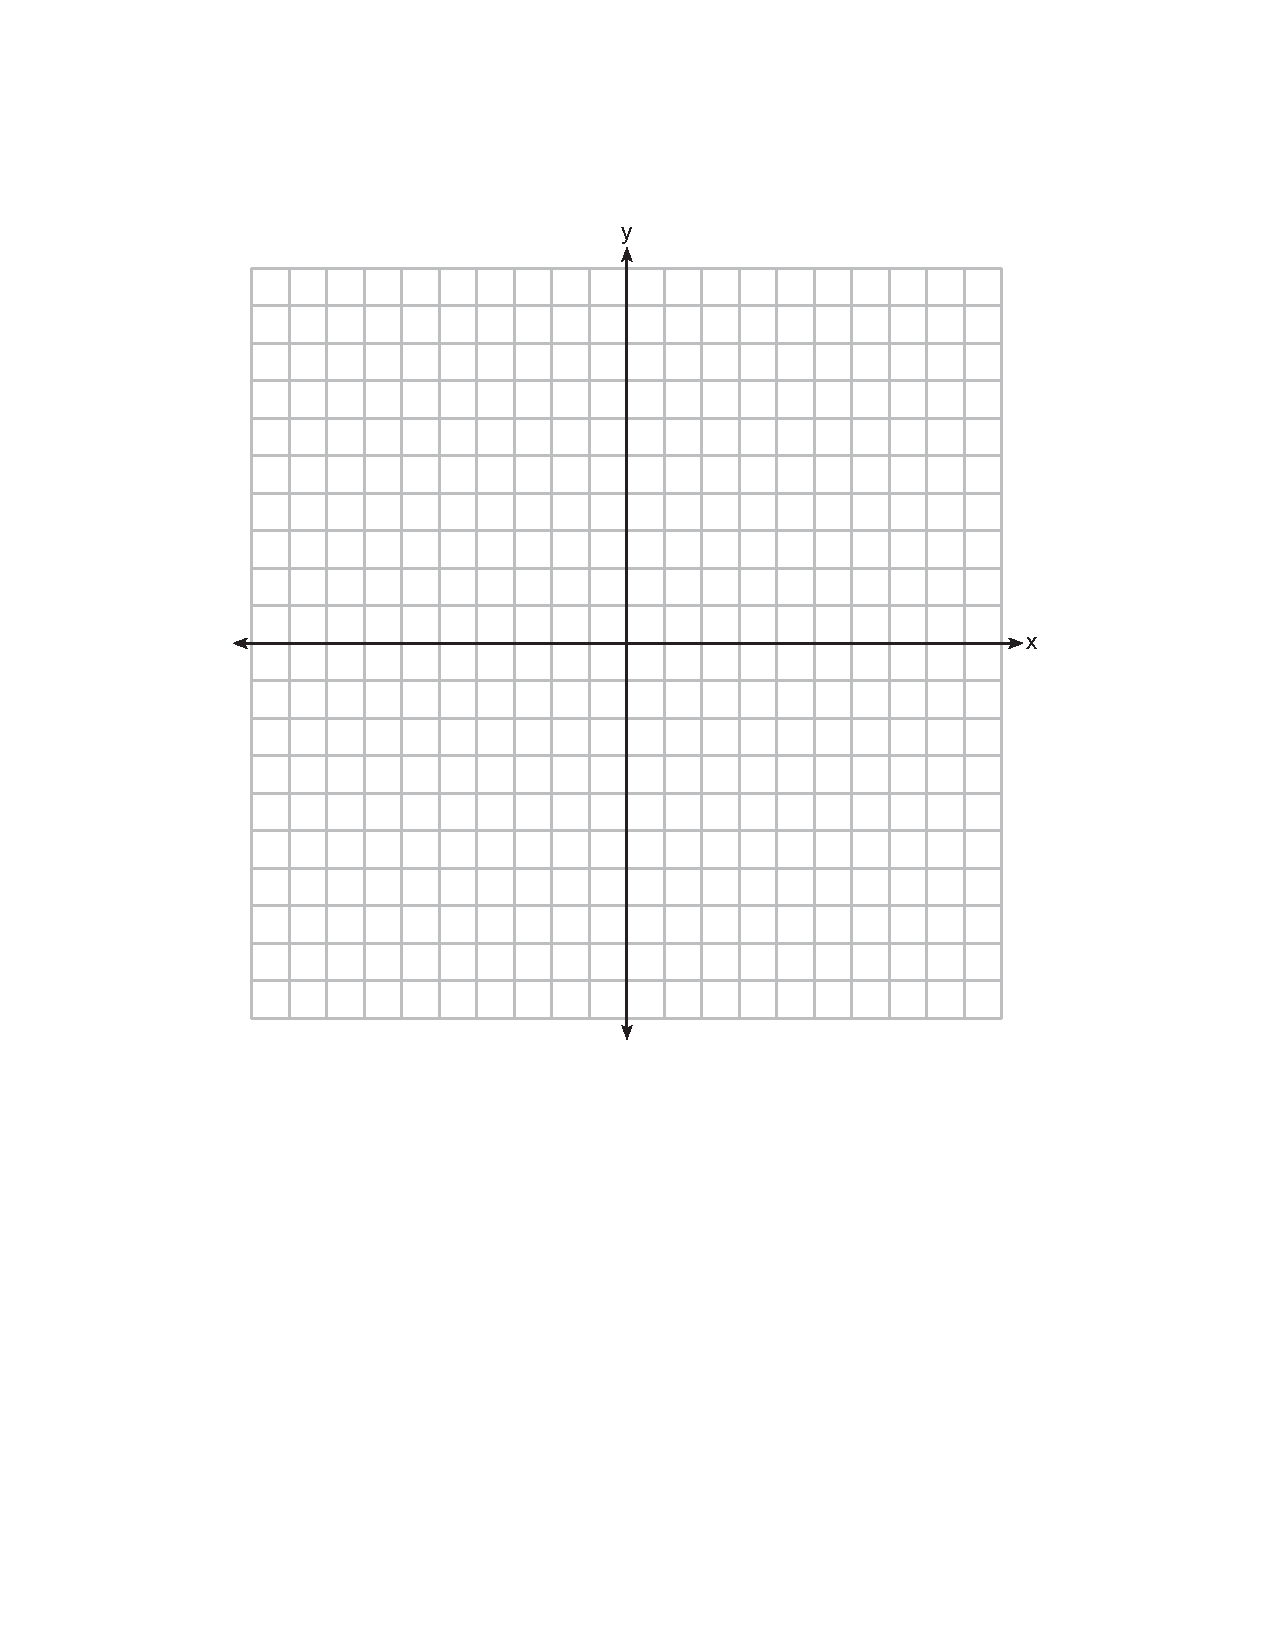
\includegraphics[width=0.75\textwidth]{regents-grid.pdf}
\end{figure}

\item Given the function $f(x)=x^3-5x^2-4x+20$. 
\begin{enumerate}
    \item Find the zeros of $f$.\\*[10pt]
    \item Write down $f(x)$ in factored form.\\*[50pt]
    \item Graph the function on the grid below, carefully passing through the correct $x-$ and $y$-intercepts. 
\end{enumerate}
\begin{center}
    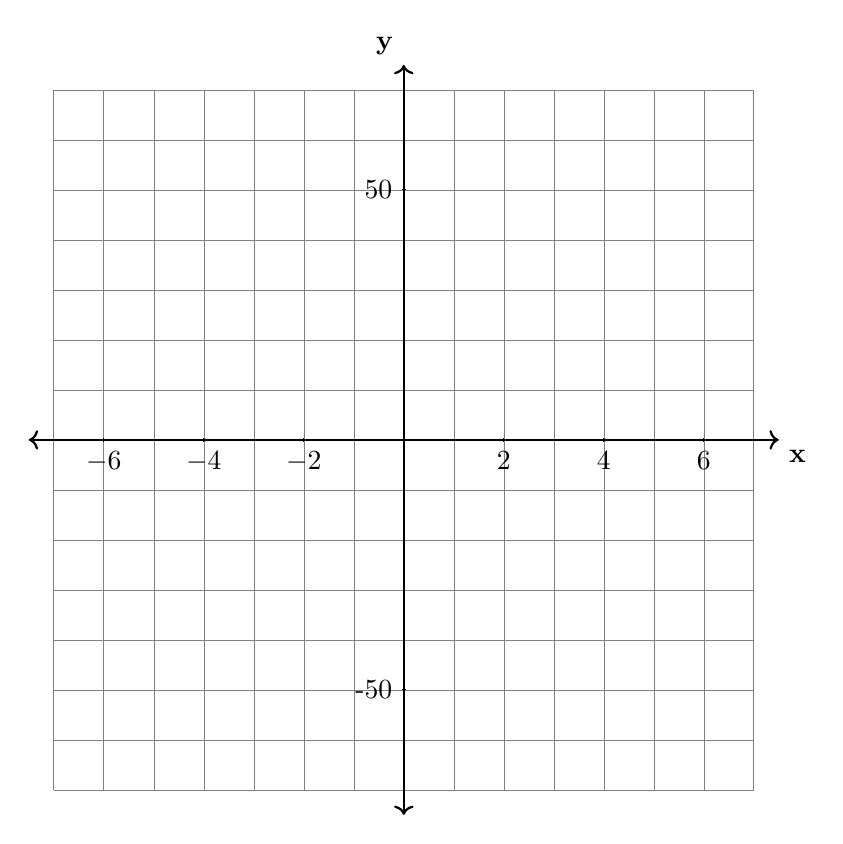
\begin{tikzpicture}[scale=2.54/4]
    \draw[step=1cm,gray,very thin] (-7,-7) grid (7,7);
    \draw[thick,<->] (-7.5,0) -- (7.5,0) node[anchor=north west] {\textbf{x}};
    \draw[thick,<->] (0,-7.5) -- (0,7.5) node[anchor=south east] {\textbf{y}};
    \foreach \x in {-6, -4, -2, 2, 4, 6} \draw (\x cm,1pt) -- (\x cm,-1pt) node[anchor=north] {$\x$};
    \foreach \y in {5} \draw (1pt,\y cm) -- (-1pt,\y cm) node[anchor=east] {50};
    \foreach \y in {-5} \draw (1pt,\y cm) -- (-1pt,\y cm) node[anchor=east] {-50};    \tkzInit[xmin=-5,xmax=5,ymin=-7,ymax=7,ystep=1]
%    \tkzFct[color=black,thick,<->,domain = -3.4:7] {0.1*(x*x-4)*(x-5)};
    \end{tikzpicture}
\end{center}

\newpage
\item Find algebraically the zeros for  $p(x)=x^3+x^2-4x-4$.\\*[1in]
On the set of axes below, graph $y=p(x)$.
\begin{center}
    
\begin{tikzpicture}[scale=2.54/4]
    \draw[step=1cm,gray,very thin] (-10,-10) grid (10,10);
    \draw[thick,<->] (-10.5,0) -- (10.5,0) node[anchor=north west] {\textbf{x}};
    \draw[thick,<->] (0,-10.5) -- (0,10.5) node[anchor=south east] {\textbf{y}};
    %\foreach \x in {-6, -4, -2, 2, 4, 6} \draw (\x cm,1pt) -- (\x cm,-1pt) node[anchor=north] {$\x$};
    %\foreach \y in {5} \draw (1pt,\y cm) -- (-1pt,\y cm) node[anchor=east] {50};
    %\foreach \y in {-5} \draw (1pt,\y cm) -- (-1pt,\y cm) node[anchor=east] {-50};    \tkzInit[xmin=-5,xmax=5,ymin=-7,ymax=7,ystep=1]
%    \tkzFct[color=black,thick,<->,domain = -3.4:7] {0.1*(x*x-4)*(x-5)};
    \end{tikzpicture}
\end{center} %Alg2 Regents Aug2016

\item Given the function $f(x)=x^3-4x^2-4x-7$. 
\begin{enumerate}
    \item Using the calculator table function, complete the $y$ values.
    \begin{tabular}{r|r}
    x & f(x)\\ 
    \hline 
    $-4$ & \\[5pt]
    $-3$ & \\[5pt]
    $-2$ & \\[5pt]
    $-1$ & \\[5pt]
    $0$ & \\[5pt]
    $1$ & \\[5pt]
    $2$ & \\[5pt]
    $3$ & \\[5pt]
    $4$ & \\[5pt]
    $5$ & \\ 
    \end{tabular}
    \item Graph the function on the grid below.
    \item Using the calculator graph-solve function, find the roots of the function, rounded to the \emph{nearest hundredth}.
\end{enumerate}
\begin{center}
    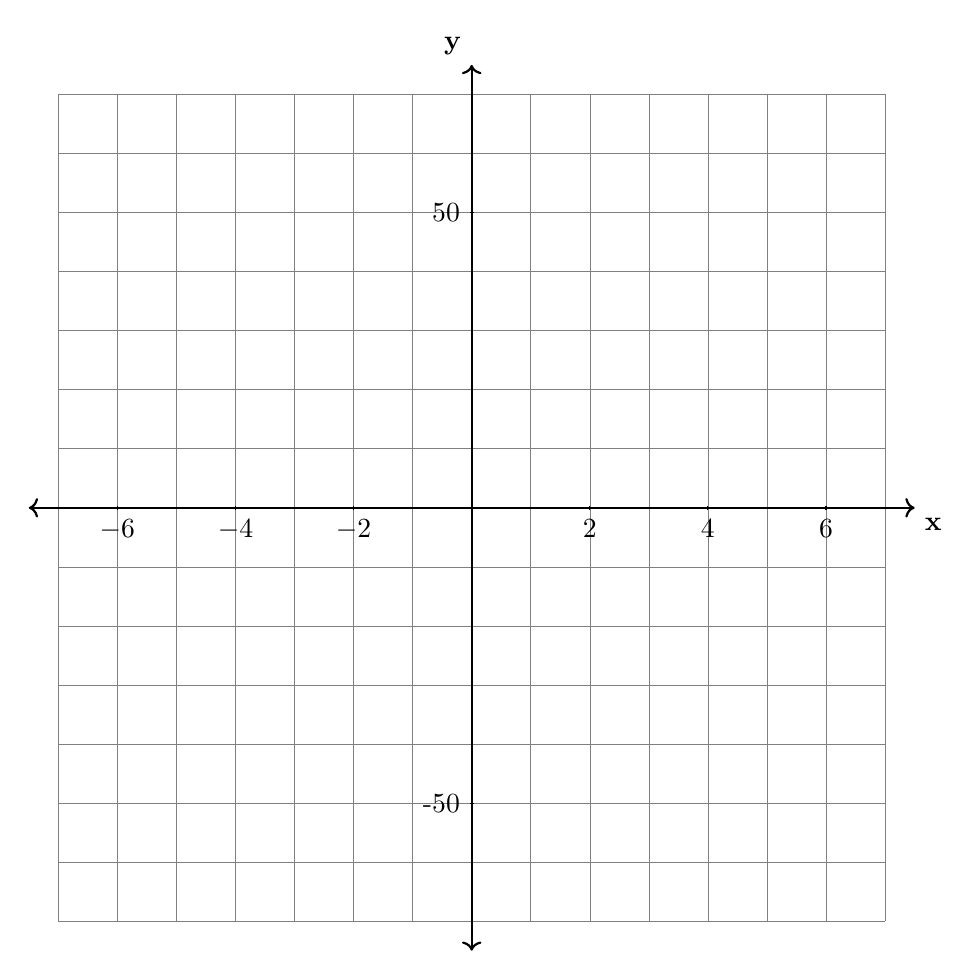
\begin{tikzpicture}[scale=3/4]
    \draw[step=1cm,gray,very thin] (-7,-7) grid (7,7);
    \draw[thick,<->] (-7.5,0) -- (7.5,0) node[anchor=north west] {\textbf{x}};
    \draw[thick,<->] (0,-7.5) -- (0,7.5) node[anchor=south east] {\textbf{y}};
    \foreach \x in {-6, -4, -2, 2, 4, 6} \draw (\x cm,1pt) -- (\x cm,-1pt) node[anchor=north] {$\x$};
    \foreach \y in {5} \draw (1pt,\y cm) -- (-1pt,\y cm) node[anchor=east] {50};
    \foreach \y in {-5} \draw (1pt,\y cm) -- (-1pt,\y cm) node[anchor=east] {-50};    \tkzInit[xmin=-5,xmax=5,ymin=-7,ymax=7,ystep=1]   
%    \tkzFct[color=black,thick,<->,domain = -3.4:7] {0.1*(x*x-4)*(x-5)};
    \end{tikzpicture}
\end{center}


\item The function below models the average price of gas in a small town since January 1st.
\[G(t)=-0.0049t^4 + 0.0923t^3 - 0.56t^2 +1.166t+3.23 \text{, where } 0 \leq t \leq 10.\]
If $G(t)$ is the average price of gas in dollars and $t$ represents the number of months since January 1st, the absolute maximum $G(t)$ reaches over the given domain is about what value, to the nearest cent? %Alg2 Regents Jan2018

\item Which graph has the following characteristics?
\begin{itemize}
\item three real zeros
\item as $x \rightarrow - \infty$, $f(x) \rightarrow - \infty$
\item as $x \rightarrow \infty$, $f(x) \rightarrow \infty$
\end{itemize}
\begin{figure}[!ht]
    \centering
    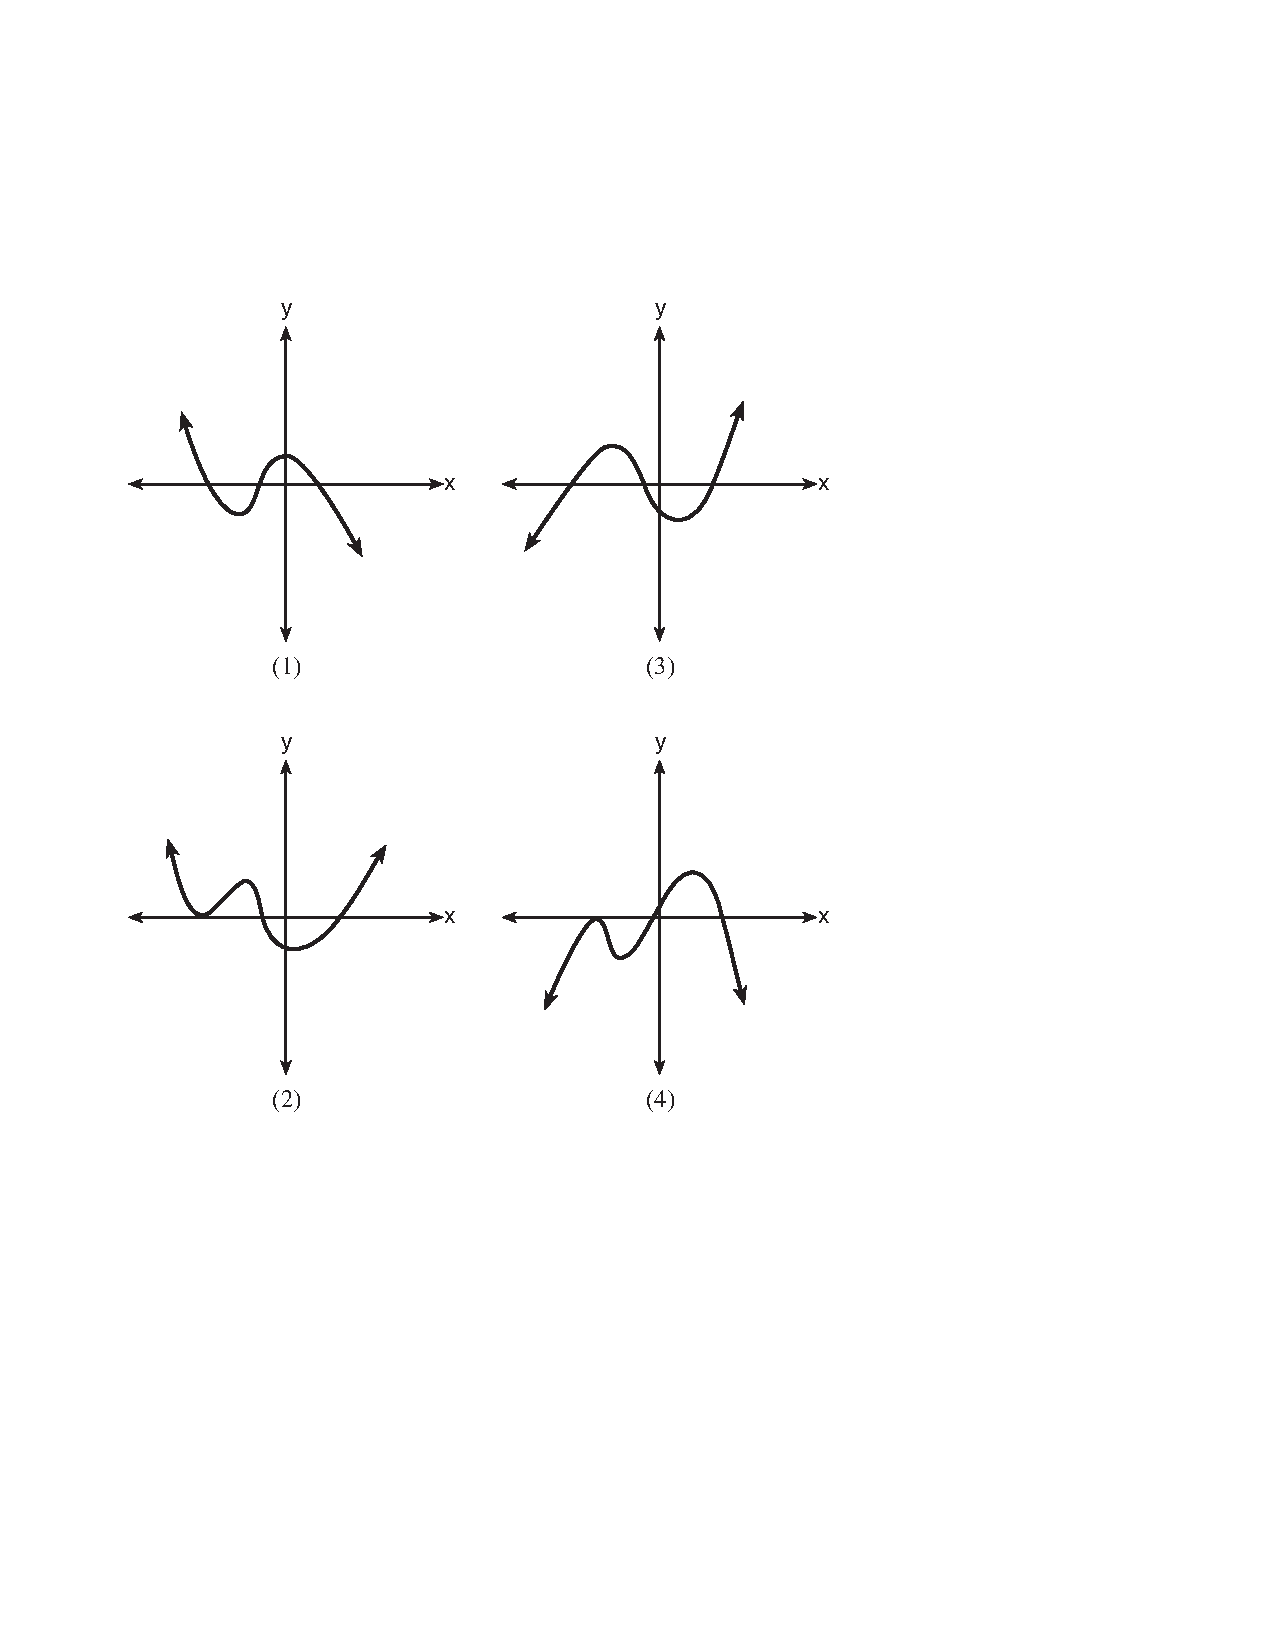
\includegraphics[width=0.75\textwidth]{cubic-graphs.pdf}
\end{figure} %Alg2 Regents Jun2016

\item Sketch a graph with the following characteristics: 
\begin{itemize}
\item three real zeros
\item as $x \rightarrow + \infty$, $f(x) \rightarrow - \infty$
\item as $x \rightarrow - \infty$, $f(x) \rightarrow + \infty$
\end{itemize}
\begin{center}
    \begin{tikzpicture}[scale=2.54/4]
    \draw[thick,<->] (-7.5,0) -- (7.5,0) node[anchor=north west] {\textbf{x}};
    \draw[thick,<->] (0,-7.5) -- (0,7.5) node[anchor=south east] {\textbf{y}};
    \end{tikzpicture}
\end{center} %Alg2 Regents Jun2016 MC


\item Sketch a graph with the following characteristics: 
\begin{itemize}
\item polynomial function of order four
\item a positive leading coefficient
\item four real zeros
\end{itemize}
\begin{center}
    \begin{tikzpicture}[scale=2/4]
    \draw[thick,<->] (-7.5,0) -- (7.5,0) node[anchor=north west] {\textbf{x}};
    \draw[thick,<->] (0,-7.5) -- (0,7.5) node[anchor=south east] {\textbf{y}};
    \end{tikzpicture}
\end{center}

\item The graph of the function $p(x)$ is sketched below.
\begin{center}
    \begin{tikzpicture}[scale=2.54/4]
    \draw[thick,<->] (-4.5,0) -- (5.5,0) node[anchor=north west] {\textbf{x}};
    \draw[thick,<->] (0,-3.5) -- (0,7.5) node[anchor=south east] {\textbf{p(x)}};
    \foreach \x in {-1, 1} \draw (\x cm,5pt) -- (\x cm,-5pt) node[anchor=north] {$\x$};
    \foreach \x in {-4,-3,-2, 2, 3, 4} \draw (\x cm,5pt) -- (\x cm,-5pt) node[anchor=north] {};
    %\foreach \y in {5} \draw (1pt,\y cm) -- (-1pt,\y cm) node[anchor=east] {50}; %{$\y$};
    \tkzInit[xmin=-5,xmax=5,ymin=-7,ymax=7,ystep=1]   
    \tkzFct[color=black,very thick,<->,domain = -3.2:4] {0.2*(x*x-9)*(x-2)};
    \end{tikzpicture}
\end{center}
Which equation could represent $p(x)$?
\begin{enumerate}
    \item $p(x)=(x^2- 9)(x-2)$
    \item $p(x)=x^3 -2x^2+ 9x+18$
    \item $p(x)=(x^2+ 9)(x-2)$
    \item $p(x)=x^3 +2x^2- 9x-18$
\end{enumerate} %Alg2 Regents Jun2017 multiple choice

\item On the axes below, sketch a possible function $p(x) = (x  -a)(x - b)(x + c)$, where $a$, $b$, and $c$ are positive, $a  >b$, and $p(x)$ has a positive $y$-intercept of $d$. Label all intercepts. 
\begin{center}
    \begin{tikzpicture}[scale=2.54/4]
    \draw[thick,<->] (-7.5,0) -- (7.5,0) node[anchor=north west] {\textbf{x}};
    \draw[thick,<->] (0,-7.5) -- (0,7.5) node[anchor=south east] {\textbf{y}};
    \end{tikzpicture}
\end{center} %Alg2 Regents Aug2017

\item The zeros of a quartic polynomial function $h$ are  $-1,\pm 2, \text{ and } 3$. Sketch a graph of $y = h(x)$ on the grid below.\\*
\begin{center}
    
\begin{tikzpicture}
    \draw[step=0.25in,gray,very thin] (0,0) grid (12.7,12.7);
    \end{tikzpicture}
\end{center}

\item The zeros of a cubic polynomial function $f$ are  $-1,2, \text{ and } 3$. Sketch a graph of $y = f(x)$ on the grid below.\\*
\begin{center}
    
\begin{tikzpicture}
    \draw[step=0.25in,gray,very thin] (0,0) grid (12.7,12.7);
    \end{tikzpicture}
\end{center}

\item On the grid below, sketch a cubic polynomial whose zeros are 1, 3, and $-2$.\\*
\begin{center}
    
\begin{tikzpicture}
    \draw[step=0.25in,gray,very thin] (0,0) grid (12.7,12.7);
    \end{tikzpicture}
\end{center} %Alg2 Regents Jan2018

\newpage
Difficulty=6
\item The graph of $y = f(x)$ is shown below. The function has a leading coefficient of 1.\\*
\begin{center}
    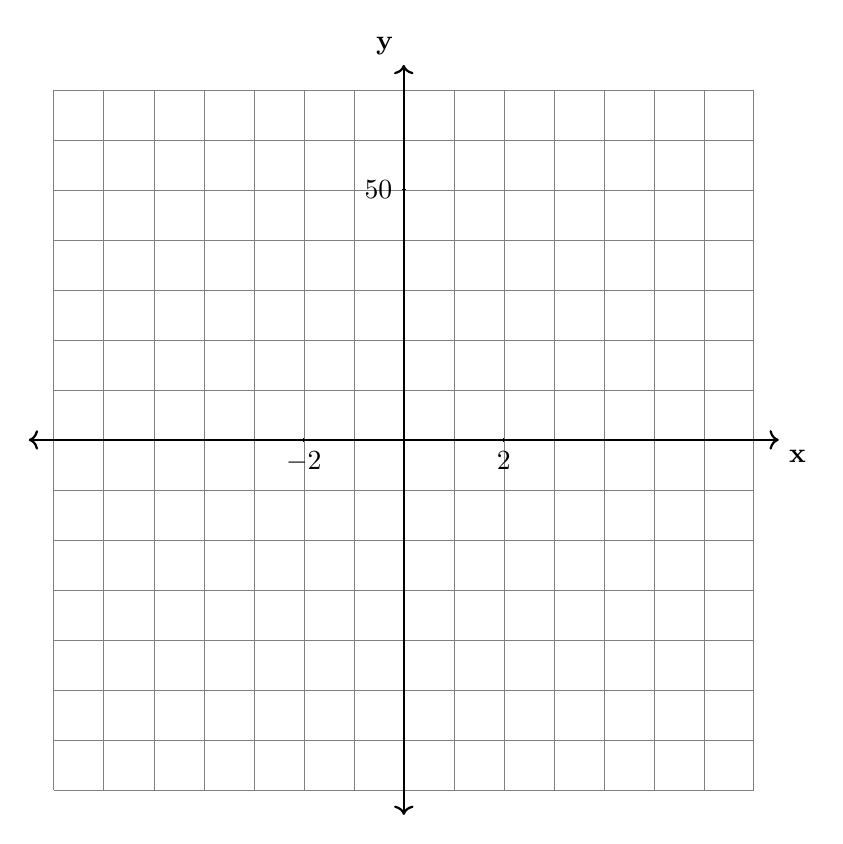
\begin{tikzpicture}[scale=2.54/4]
    \draw[step=1cm,gray,very thin] (-7,-7) grid (7,7);
    \draw[thick,<->] (-7.5,0) -- (7.5,0) node[anchor=north west] {\textbf{x}};
    \draw[thick,<->] (0,-7.5) -- (0,7.5) node[anchor=south east] {\textbf{y}};
    \foreach \x in {-2, 2} \draw (\x cm,1pt) -- (\x cm,-1pt) node[anchor=north] {$\x$};
    \foreach \y in {5} \draw (1pt,\y cm) -- (-1pt,\y cm) node[anchor=east] {50}; %{$\y$};
    \tkzInit[xmin=-5,xmax=5,ymin=-7,ymax=7,ystep=1]   
    \tkzFct[color=black,thick,<->,domain = -4.4:3.6] {0.1*(x+4)*x*x*(x-3)};
    \end{tikzpicture}
\end{center}
Write an equation for $f(x)$.\\*[10pt]
The function $g$ is formed by translating function $f$ left 2 units. Write an equation for $g(x)$.

\item The graph of $y = f(x)$ is shown below. The function has a leading coefficient of 1.\\*
\begin{center}
    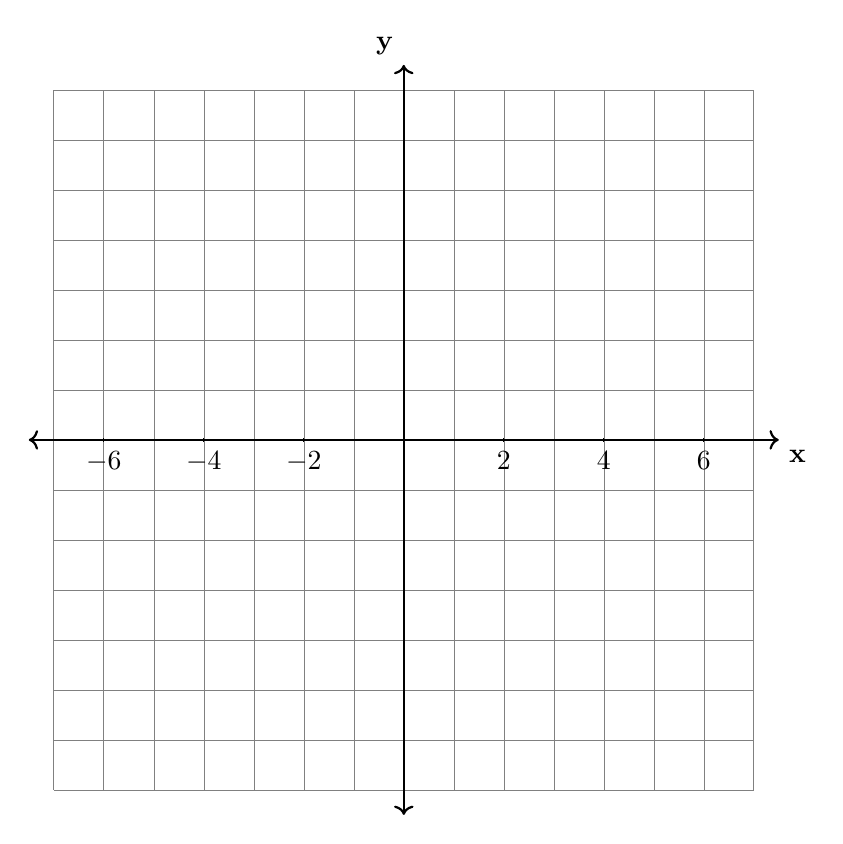
\begin{tikzpicture}[scale=2.54/4]
    \draw[step=1cm,gray,very thin] (-7,-7) grid (7,7);
    \draw[thick,<->] (-7.5,0) -- (7.5,0) node[anchor=north west] {\textbf{x}};
    \draw[thick,<->] (0,-7.5) -- (0,7.5) node[anchor=south east] {\textbf{y}};
    \foreach \x in {-6, -4, -2, 2, 4, 6} \draw (\x cm,1pt) -- (\x cm,-1pt) node[anchor=north] {$\x$};
    %\foreach \y in {5} \draw (1pt,\y cm) -- (-1pt,\y cm) node[anchor=east] {50}; %{$\y$};
    \tkzInit[xmin=-6,xmax=5,ymin=-7,ymax=7,ystep=1]   
    \tkzFct[color=black,thick,<->,domain = -5.3:4.2] {0.1*(x+4)*(x+1)*(x-3)};
    \end{tikzpicture}
\end{center}
Write an equation for $f(x)$.\\*[10pt]
The function $g$ is formed by translating function $f$ left 3 units. Write an equation for $g(x)$.


\item A polynomial equation of degree three, $p(x)$, is used to model the volume of a rectangular box. The graph of $p(x)$ has $x$ intercepts at  $-2$, 10, and 14. Which statements regarding $p(x)$ could be true?\\*
A. The equation of $p(x) = (x - 2)(x + 10)(x +14)$.\\*
B. The equation of $p(x) = -(x + 2)(x - 10)(x - 14)$.\\*
C. The maximum volume occurs when $x = 10$.\\*
D. The maximum volume of the box is approximately 56.\\* %Alg2 Regents Aug2017 multiple choice

\item Algebraically determine whether the function $j(x) = x^4- 3x^2- 4$ is odd, even, or neither. %Alg2 Regents Aug2017

\subsubsection*{Topic="Polynomial Identities"\\
Source="Regents" 
Difficulty=5}

\item Given: $f(x)=2x^2+ x - 3$ and $g(x)=x-1$\\*[5pt]
Express $f(x) \bullet g(x) - [f(x) + g(x)]$ as a polynomial in standard form. %Alg2 Regents Jan2018

\item Given: $f(x)=x^2+ x - 2$ and $g(x)=x-1$\\*[5pt]
Express $2 \bullet g(x) - f(x)$ as a polynomial in standard form. %Alg2 Regents Jan2018

\item If $p(x)=ab^x$ and $r(x)=cd^x$, then $p(x) \bullet r(x)$ equals
\begin{enumerate}
    \item $ac(b+d)^x$
    \item $ac(b+d)^{2x}$
    \item $ac(bd)^x$
    \item $\displaystyle ac(bd)^{x^2}$
\end{enumerate} %Regents Alg2 Jan2017 MC


\item If $g(c)=1-c^2$ and $m(c)=c+1$, then which statement is \emph{not} true?
\begin{enumerate}
    \item $g(c) \bullet m(c) = 1+c-c^2-c^3$
    \item $g(c) + m(c) = 2+c-c^2$
    \item $m(c) - g(c) = c+c^2$
    \item $\displaystyle \frac{m(c)}{g(c)} = \frac{-1}{1-c}$
\end{enumerate} %Regents Alg2 Jun2016


\item Algebraically determine the values of $h$ and $k$ to correctly complete the identity stated below.
\[2x^3-10x^2+11x-7=(x-4)(2x^2+hx+3)+k\] %Alg2 Regents Jan 2017

\item Algebraically determine the values of $h$ and $k$ to correctly complete the identity stated below.
\[10x^2-11x-7=(x-2)(hx+9)+k\]

\item Algebraically determine the values of $h$ and $k$ to correctly complete the identity stated below.
\[2x^3-5x^2+12x-5=(2x-1)(x^2-hx+k)\]

\item The expression $(x + a)(x + b)$ can not be written as
\begin{enumerate}
    \item $a(x + b)+ x(x + b)$
    \item $x^2 + (a + b)x + ab$ 
    \item  $x^2 + abx + ab$  
    \item $x(x + a)+ b(x + a)$
\end{enumerate}

Difficulty=6
\item Verify the following Pythagorean identity for all values of $x$ and $y$: \[(x^2 + y^2)^2= (x^2- y^2)^2+ (2xy)^2\] %Alg2 Regents Aug2017

\item A manufacturing company has developed a cost model, $C(x)=0.15x^3+0.01x^2+2x+120$, where $x$ is the number of items sold, in thousands. The sales price can be modeled by $S(x)=30-0.01x$. Therefore, revenue is modeled by $R(x)=x \cdot S(x)$.\\*[5pt]
The company’s profit, $P(x)=R(x)-C(x)$, could be modeled by what polynomial?  %Alg2 Regents Jun2017 multiple choice

\item Sally’s high school is planning their spring musical. The revenue, $R$, generated can be determined by the function $R(t)=-33t^2+360t$, where $t$ represents the price of a ticket. The production cost, $C$, of the musical is represented by the function $C(t)=700+5t$. What is the highest ticket price, to the \emph{nearest dollar}, they can charge in order to not lose money on the event? %Alg2 Regents Aug2016 multiple choice

Difficulty=4
\item What is the quotient when $x^2-3x-40$ is divided by $x + 5$?
\item What is the quotient when $x^3+3x^2-x+2$ is divided by $x - 1$?
\item What is the quotient when $3x^3+9x^2+8x+5$ is divided by $x+2$?
\item What is the quotient when $x^3-13x-12$ is divided by $x - 4$?
\item What is the quotient when $10x^3-3x^2-7x+3$ is divided by $2x - 1$? %Jan2018 Regents multiple choice

\item Determine whether the binomial $x+2$ is a factor of $f(x)=x^3+x^2-16x-16$
\item Determine whether the binomial $x+3$ is a factor of $f(x)=3x^3+10x^2-x-12$

\item Determine if $x-5$ is a factor of $2x^3-4x^2-7x-10$. Explain your answer. %Jun2016 Regents FR

\item Given that $x-2$ is a factor of $f(x)=3x^3-9x^2+8x-4$. What is the value of $f(2)$?

\item When $g(x)$ is divided by $x+4$, the remainder is 0. Given $g(x)= x^4+3x^3-6x^2-6x+8$, which conclusion about $g(x)$ is true?
\begin{enumerate}
    \item $g(4)=0$
    \item $g(-4)=0$
    \item $x-4$ is a factor of $g(x)$.
    \item No conclusion can be made regarding $g(x)$.
\end{enumerate} %Alg2 Regents Jan2017 multiple choice

\item The graph of $p(x)$ is shown below.
\begin{center}
    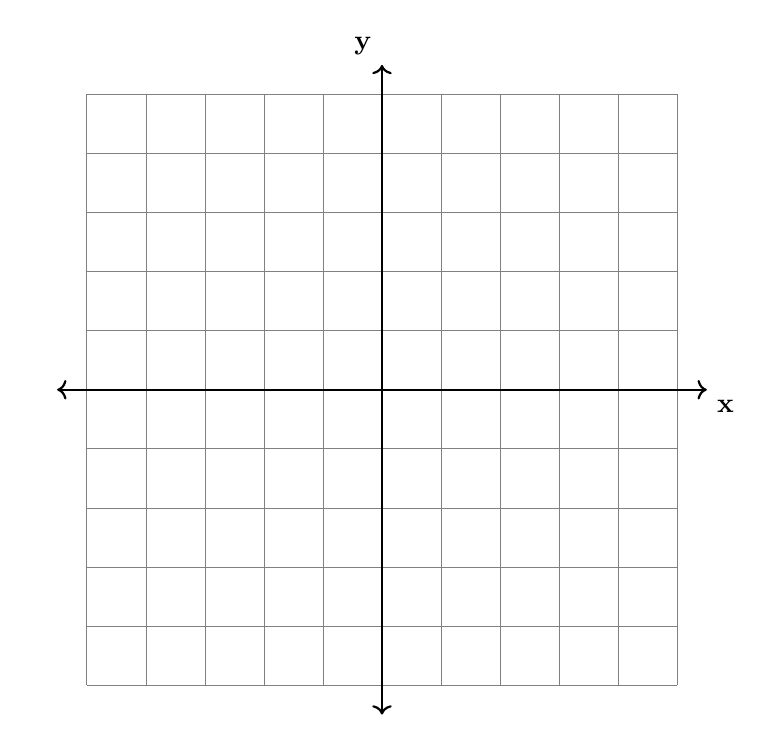
\begin{tikzpicture}[scale=3/4]
    \draw[step=1cm,gray,very thin] (-5,-5) grid (5,5);
    \draw[thick,<->] (-5.5,0) -- (5.5,0) node[anchor=north west] {\textbf{x}};
    \draw[thick,<->] (0,-5.5) -- (0,5.5) node[anchor=south east] {\textbf{y}};
    %\foreach \x in {-6, -4, -2, 2, 4, 6} \draw (\x cm,1pt) -- (\x cm,-1pt) node[anchor=north] {$\x$};
    %\foreach \y in {5} \draw (1pt,\y cm) -- (-1pt,\y cm) node[anchor=east] {50}; %{$\y$};
    \tkzInit[xmin=-6,xmax=5,ymin=-5,ymax=5,ystep=1]   
    \tkzFct[color=black,thick,<->,domain = -4.6:3.7] {0.2*(x+4)*(x)*(x-3)};
    \end{tikzpicture}
\end{center}
What is the remainder when $p(x)$ is divided by $x+4$? %Alg2 Regents Aug2016 multiple choice

\item Which binomial is a factor of $x^4-4x^2-4x+8$?
\begin{enumerate}
    \item $x-2$
    \item $x+2$
    \item $x-4$
    \item $x+4$
\end{enumerate} %Alg2 Regents Jun2017 multiple choice


\item Which binomial is \emph{not} a factor of the expression $x^3- 11x^2 +16x +84$?
\begin{enumerate}
    \item $x+2$
    \item $x-6$
    \item $x+4$
    \item $x-7$
\end{enumerate}

\item The expression $\displaystyle \frac{x^3+2x^2+x+6}{x+2}$ is equivalent to \begin{enumerate}
    \item $x^2+3$
    \item $\displaystyle x^2+1+\frac{4}{x+2}$
    \item $2x^2+x+6$
    \item $\displaystyle 2x^2+1+\frac{4}{x+2}$
\end{enumerate}
%Alg2 Regents Aug2016 multiple choice

\item The expression $\displaystyle \frac{4x^3+5x+10}{2x+3}$ is equivalent to \begin{enumerate}
    \item $\displaystyle 2x^2+3x-7+\frac{31}{2x+3}$
    \item $\displaystyle 2x^2-3x+7-\frac{11}{2x+3}$
    \item $\displaystyle 2x^2+2.5x+5+\frac{15}{2x+3}$
    \item $\displaystyle 2x^2-2.5x-5-\frac{20}{2x+3}$
\end{enumerate} %Alg2 Regents Jun2016 multiple choice

\item Simplify the expression $\displaystyle \frac{4x^3+9x-5}{2x-1}$, where $x \neq \frac{1}{2}$. %Alg2 Regents Aug2017 multiple choice

\item Given $f(x)=3x^2+7x-20$ and $g(x)=x-2$, state the quotient and remainder of $\displaystyle \frac{f(x)}{g(x)}$, in the form $\displaystyle q(x)+ \frac{r(x)}{g(x)}$. %Alg2 Regents Jan2017

\item If $p(x)=2x^3-3x+5$, what is the remainder of $p(x) \div (x-5)$? %Alg2 Regents Jan2018 multiple choice

\item Use long division to determine the quotient and remainder of $(x^3+4x^2-8x-6) \div (x+2)$.
\item Use long division to determine the quotient and remainder of $(x^3-7x^2+15x-9) \div (x-3)$.
\item Use long division to determine the quotient and remainder of $(x^3+4x^2-8x-6) \div (x+2)$.

\item Given that the remainder when  $f(x)=x^3-3x^2+2x+125$ is divided by $x+4$ is $-5$. What is the value of $f(-4)$?

\item Given $r(x)=x^3-4x^2+4x-6$, find the value of $r(2)$.\\*[15pt]
What does your answer tell you about $x-2$ as a factor of $r(x)$? Explain. %Alg2 Regents Jun2017 

\item Over the set of integers, factor the expression $4x^3-x^2  +16x-4$ completely.
 %Alg2 Regents Jun2017 complex roots, leave as integers
 
\subsubsection*{Topic="Solving Linear Systems"\\
Source="Regents" 
Difficulty=5}

\item Solve the following system of equations:
\[y=-2x+14\]
\[3x - 4z = 2\]
\[3x - y  = 16\]

\item Solve the following system of equations algebraically for all values of $x$, $y$, and $z$:
\[x +y+ z=1\]
\[2x+4y+6z=2\]
\[-x+3y-5z=11\]
(Note: requires algebraic work, perhaps matrix notation would do)

\subsubsection*{Topic="Modeling Rationals"\\
Source="Regents" 
Difficulty=5}

\item Mallory wants to buy a new window air conditioning unit. The cost for the unit is \$329.99. If she plans to run the unit three months out of the year for an annual operating cost of \$108.78, which function models the cost per year over the lifetime of the unit, $C(n)$, in terms of the number of years, $n$, that she owns the air conditioner?
\begin{enumerate}
    \item $C(n)=329.99+108.78n$
    \item $C(n)=329.99+326.34n$
    \item $\displaystyle C(n)=\frac{329.99+108.78n}{n}$
    \item $\displaystyle C(n)=\frac{329.99+326.34n}{n}$
\end{enumerate} %Alg2 Regents Jun2017 multiple choice

\subsubsection*{Topic="Operations with Complex Numbers"\\
Source="Regents" 
Difficulty=5}

\item Express $(1-i)^3$ in $a+bi$ form. %Alg2 Regents Jan2017

\item What is the expression $6xi^3(-4xi+5)$ is equivalent to?  %Alg2 Regents Jun2017 multiple choice

\item Given $i$ is the imaginary unit, $(2-yi)^2$ in simplest form is what? %Alg2 Regents Jun2016

\item Simplify the expression $(3k - 2i)^2$, where $i$ is the imaginary unit. %Alg2 Regents Aug2017


\item Simplify $xi(i - 7i)^2$, where $i$ is the imaginary unit. %Alg2 Regents Aug2016

\item Nicole tried to find the product of $(2+ 4i)$ and $(3 - i)$, and her work is shown below.
$(2 + 4i)(3 - i)$\\*
$=6 - 2i + 12i - 4i^2$\\*
$=6 + 10i - 4i^2$\\*
$=6 + 10i - 4(1)$\\*
$=6 + 10i - 4$\\*
$=2 + 10i$\\*
Identify the error in the process shown and determine the correct product of $(2+ 4i)$ and $(3 - i)$.%Alg2 Regents Jan2018

\subsubsection*{Topic="Radicals and Rational Exponents"\\
Source="Regents" 
Difficulty=4}

\item The solution set for the equation $\sqrt{x+14}- \sqrt{2x+5}= 1$ is
\begin{enumerate}
    \item \{-6\}
    \item \{2\}
    \item \{18\}
    \item \{2, 22\}
\end{enumerate} %Alg2 Regents Aug2017 multiple choice

\item Solve algebraically for all values of $x$: 
\[\sqrt{x-4}+x=6\] %Alg2 Regents Jun2017


Difficulty=5
\item Write $\sqrt[3]x \cdot \sqrt{x}$ as a single term with a rational exponent. %Alg2 Regents Jun2017

\item What does $\displaystyle \left( \frac{-54x^9}{y^4} \right)^\frac{2}{3}$ equal? %Alg2 Regents Aug2017 multiple choice

\item The expression $\displaystyle \left( \frac{m^2}{m^\frac{1}{3}}\right)^{-\frac{1}{2}}$ is equivalent to 
\begin{enumerate}
    \item $-\sqrt[6]{m^5}$
    \item $\displaystyle \frac{1}{\sqrt[6]{m^5}}$
    \item $-m \sqrt[5]{m}$
    \item $\displaystyle \frac{1}{m \sqrt[5]{m}}$
\end{enumerate} %Alg2 Regents Jan2017 multiple choice

\item When $b>0$ and $d$ is a positive integer, the expression $\displaystyle \left(3b \right)^\frac{2}{d}$ is equivalent to what expressed as a radical? %Alg2 Regents Jun2016 multiple choice


\item For $x \neq 0$, which expressions are equivalent to one divided by the sixth root of $x$?
\begin{center}
    I. $\frac{\sqrt[6]{x}}{\sqrt[3]{x}}$ \qquad  II. $\displaystyle \frac{x^\frac{1}{6}}{x^\frac{1}{3}}$  \qquad  III. $x^{-\frac{1}{6}}$
\end{center}


\item Explain how $\displaystyle (-8)^\frac{4}{3}$ can be evaluated using properties of rational exponents to result in an integer answer.

\item Explain how $\displaystyle \left(3^{\frac{1}{5}} \right)^2$ can be written as the equivalent radical expression $\sqrt[5]9$. %Alg2 Regents Aug2016

\item Explain why $81^\frac{3}{4} \text{ equals } 27$.

\item Given the equal terms $\displaystyle \sqrt[3]{x^5}$ and $\displaystyle y^{\frac{5}{6}}$, determine and state $y$, in terms of $x$. %Alg2 Regents Jan2017

\newpage
\subsubsection*{Topic="Powers of Powers"\\
Source="Regents" 
Difficulty=6}

\item If $n=\sqrt{a^5}$ and $m=a$, where $a > 0$, express $\frac{n}{m}$ as 
\begin{enumerate}
    \item a radical with positive, integer exponents
    \item an expression with a fractional exponent
\end{enumerate}

\item According to a pricing website, Indroid phones lose 58\% of their cash value over 1.5 years. Which expression can be used to estimate the value of a \$300 Indroid phone in 1.5 years?
\begin{enumerate}
    \item $300e^{-0.87}$
    \item $300e^{-0.63}$
    \item $300e^{-0.58}$
    \item $300e^{-0.42}$
\end{enumerate} %Alg2 Regents Jan2017 MC


\item The function $p(t)=110e^{0.03922t}$ models the population of a city, in millions, $t$ years after 2010. As of today, consider whether the following two statements are true or false:
\begin{enumerate}
    \item The current population is 110 million.
    \item The population increases continuously by approximately 3.9\% per year.
\end{enumerate} %Alg2 Regents Jun2017 multiple choice

\item Last year, the total revenue for Home Style, a national restaurant chain, increased 5.25\% over the previous year. If this trend were to continue, which expression could the company’s chief financial officer use to approximate their monthly percent increase in revenue? [Let $m$ represent months.]
\begin{enumerate}
    \item $(1.0525)^m$
    \item $\displaystyle (1.0525)^{\frac{12}{m}}$
    \item $(1.00427)^m$
    \item $\displaystyle (1.00427)^{\frac{m}{12}}$
\end{enumerate} %Alg2 Regents Jun2016 multiple choice

\item For a given time, $x$, in seconds, an electric current, $y$, can be represented by $y = 2.5(1 - 2.7^{-.10x})$. Which equation is \emph{not} equivalent?
\begin{enumerate}
    \item $y = 2.5 - 2.5 (2.7^{-.10x})$
    \item $y = 2.5 - 2.5 ((2.7^2)^{-.05x})$
    \item $\displaystyle y = 2.5 - 2.5 \left( \frac{1}{2.7^{.10x}} \right)$
    \item $y = 2.5 - 2.5 (2.7^{-2})(2.7^{.05x})$
\end{enumerate}

\item Iridium-192 is an isotope of iridium and has a half-life of 73.83 days. If a laboratory experiment begins with 100 grams of Iridium-192, the number of grams, $A$, of Iridium-192 present after $t$ days would be 
\[A=100 \left( \frac{1}{2} \right)^\frac{t}{73.83}\]
Which equation approximates the amount of Iridium-192 present after $t$ days?
\begin{enumerate}
    \item $\displaystyle A=100 \left( \frac{73.83}{2} \right)^t$
    \item $\displaystyle A=100 \left( \frac{1}{147.66} \right)^t$
    \item $A=100  (0.990656)^t$
    \item $A=100 (0.116381)^t$
\end{enumerate}

\item A student studying public policy created a model for the population of Detroit, where the population decreased 25\% over a decade. He used the model $P =714(0.75)^d$, where $P$ is the population, in thousands, $d$ decades after 2010. Another student, Suzanne, wants to use a model that would predict the population after $y$ years. Suzanne’s model is best represented by
\begin{enumerate}
    \item $P=714(0.6500)^y$
    \item $P=714(0.8500)^y$
    \item $P=714(0.9716)^y$
    \item $P=714(0.9750)^y$
\end{enumerate}  %Alg2 Regents Jun2017 multiple choice


\subsubsection*{Topic="Exponential Equations, Exponential Growth, Exponential Decay"\\
Source="Regents" 
Difficulty=5 (note: exponential regression problems}

\item If the function $g(x) = ab^x$ represents exponential growth, which statement about $g(x)$ is false?
\begin{enumerate}
    \item $a > 0$ and $b>1$
    \item The $y$-intercept is $(0, a)$.
    \item The asymptote is $y=0$.
    \item The $x$-intercept is $(b,0)$
\end{enumerate} %Alg2 Regents Jan2018 multiple choice

\item A certain pain reliever is taken in 220 mg dosages and has a half-life of 12 hours. The function $\displaystyle A = 220 \left( \frac{1}{2} \right) ^\frac{t}{12}$ can be used to model this situation, where $A$ is the amount of pain reliever in milligrams remaining in the body after $t$ hours.\\*
According to this function, which statement is true?
\begin{enumerate}
    \item Every hour,the amount of pain reliever remaining is cut in half. 
    \item In 12 hours, there is no pain reliever remaining in the body.
    \item In 24 hours, there is no pain reliever remaining in the body.
    \item In 12 hours, 110 mg of pain reliever is remaining.
\end{enumerate}

\item Which function represents exponential decay?
\begin{enumerate}
    \item $y=2^{0.3t}$
    \item $y=1.2^{3t}$
    \item $\displaystyle y=\left( \frac{1}{2}\right) ^{-t}$
    \item $y=5^{-t}$
\end{enumerate} %Alg2 Regents Jun2016

\item The function $M(t)$ represents the mass of radium over time, $t$, in years.
\[M(t)=100e^{\frac{\left(\ln{\frac{1}{2}}\right)t}{1590}}
\]
Determine if the function $M(t)$ represents growth or decay. Explain your reasoning. %Alg2 Regents Jan2017

\item One of the medical uses of Iodine–131 (I–131), a radioactive isotope of iodine, is to enhance x-ray images. The half-life of I–131 is approximately 8.02 days. A patient is injected with 20 milligrams of I–131. Determine, to the \emph{nearest day}, the amount of time needed before the amount of I–131 in the patient’s body is approximately 7 milligrams. %Alg2 Regents Aug2016

\item An equation to represent the value of a car after $t$ months of ownership is $\displaystyle v=32,000(0.81)^{\frac{t}{12}}$. Which statement is \emph{not} correct?
\begin{enumerate}
    \item The car lost approximately 19\% of its value each month.
    \item The car maintained approximately 98\% of its value each month.
    \item The value of the car when it was purchased was \$32,000.
    \item The value of the car 1 year after it was purchased was \$25,920.
\end{enumerate} %Alg2 Regents Aug2016 MC

\item A payday loan company makes loans between \$100 and \$1000 available to customers. Every 14 days, customers are charged 30\% interest with compounding. In 2013, Remi took out a \$300 payday loan. Which expression can be used to calculate the amount she would owe, in dollars, after one year if she did not make payments?
\begin{enumerate}
    \item $\displaystyle 300(.30)^{ \frac{14}{365}}$
    \item $\displaystyle 300(1.30)^{ \frac{14}{365}}$
    \item $\displaystyle 300(.30)^{ \frac{365}{14}}$
    \item $\displaystyle 300(1.30)^{ \frac{365}{14}}$
\end{enumerate} %Alg2 Regents Aug2016 MC

\item Judith puts \$5000 into an investment account with interest compounded continuously. What is the approximate annual rate is needed for the account to grow to \$9110 after 30 years?

\item Jasmine decides to put \$100 in a savings account each month. The account pays 3\% annual interest, compounded monthly. How much money, $S$, will Jasmine have after one year?
\begin{enumerate}
    \item $S=100(1.03)^{12}$
    \item $\displaystyle S=\frac{100-100(1.0025)^{12}}{1-1.0025}$
    \item $S=100(1.0025)^{12}$
    \item $\displaystyle S=\frac{100-100(1.03)^{12}}{1-1.03}$
\end{enumerate} %Alg2 Regents Jun2017 multiple choice

\item Jim is looking to buy a vacation home for \$172,600 near his favorite southern beach. The formula to compute a mortgage payment, $M$, is $\displaystyle M=P \cdot \frac{r(1+r)^N}{(1+r)^N-1}$ where $P$ is the principal amount of the loan, $r$ is the monthly interest rate, and $N$ is the number of monthly payments. Jim’s bank offers a monthly interest rate of 0.305\% for a 15-year mortgage.\\*[5pt]
With no down payment, determine Jim’s mortgage payment, rounded to the nearest dollar.\\*[15pt]
Algebraically determine and state the down payment, rounded to the \emph{nearest dollar}, that Jim needs to make in order for his mortgage payment to be \$1100.
 %Alg2 Regents Jun2017 multiple choice
 
\item Using the formula below, determine the monthly payment on a 5-year car loan with a monthly percentage rate of 0.625\% for a car with an original cost of \$21,000 and a \$1000 down payment, to the \emph{nearest cent}.\\
$\displaystyle P_n=PMT\left( \frac{1-(1+i)^{-n}}{i} \right)$\\*[5pt]
$P_n = $ present amount borrowed \\*[5pt]
$n = $ number of monthly pay periods\\*[5pt]
$PMT=$ monthly payment\\*[5pt]
$i=$ interest rate per month\\[1in]
The affordable monthly payment is \$300 for the same time period. Determine an appropriate down payment, to the \emph{nearest dollar}. %Alg2 Regents Jan2017 

\item Seth’s parents gave him \$5000 to invest for his 16th birthday. He is considering two investment options. Option $A$ will pay him 4.5\% interest compounded annually. Option $B$ will pay him 4.6\% compounded quarterly.\\[10pt]
Write a function of option $A$ and option $B$ that calculates the value of each account after $n$ years.\\[1in]
Seth plans to use the money after he graduates from college in 6 years. Determine how much more money option $B$ will earn than option $A$ to the \emph{nearest cent}.\\[1in]
Algebraically determine, to the nearest tenth of a year, how long it would take for option $B$ to double Seth’s initial investment. %Alg2 Regents Aug2016

\item A rabbit population doubles every 4 weeks. There are currently five rabbits in a restricted area. If $t$ represents the time, in weeks, and $P(t)$ is the population of rabbits with respect to time, about how many rabbits will there be in 98 days? %Alg2 Regents Jan2017 

\item Researchers in a local area found that the population of rabbits with an initial population of 20 grew continuously at the rate of 5\% per month. The fox population had an initial value of 30 and grew continuously at the rate of 3\% per month.\\*[5pt]
Find, to the \emph{nearest tenth of a month}, how long it takes for these populations to be equal. %Alg2 Regents Jan2018

\item Pedro and Bobby each own an ant farm. Pedro starts with 100 ants and says his farm is growing exponentially at a rate of 15\% per month. Bobby starts with 350 ants and says his farm is steadily decreasing by 5 ants per month.\\[5pt]
Assuming both boys are accurate in describing the population of their ant farms, after how many months will they both have approximately the same number of ants? %Alg2 Regents Jan2017

\item In New York State, the minimum wage has grown exponentially. In 1966, the minimum wage was \$1.25 an hour and in 2015, it was \$8.75. Algebraically determine the rate of growth to the \emph{nearest percent}.

\item A radioactive substance has a mass of 140 g at 3 p.m. and 100 g at 8 p.m. Write an equation in the form $A = A_0 \left( \frac{1}{2} \right)^{\frac{t}{h}}$ that models this situation, where $h$ is the constant representing the number of hours in the half-life, $A_0$ is the initial mass, and $A$ is the mass $t$ hours after 3 p.m.\\*[10pt]
Using this equation, solve for $h$, to the \emph{nearest ten thousandth}. \\*[10pt]
Determine when the mass of the radioactive substance will be 40 g. Round your answer to the \emph{nearest tenth of an hour}.
 %Alg2 Regents Jun2017
 
\item Graph $y=400(.85)^{2x}-6$ on the set of axes below.
\begin{center}
    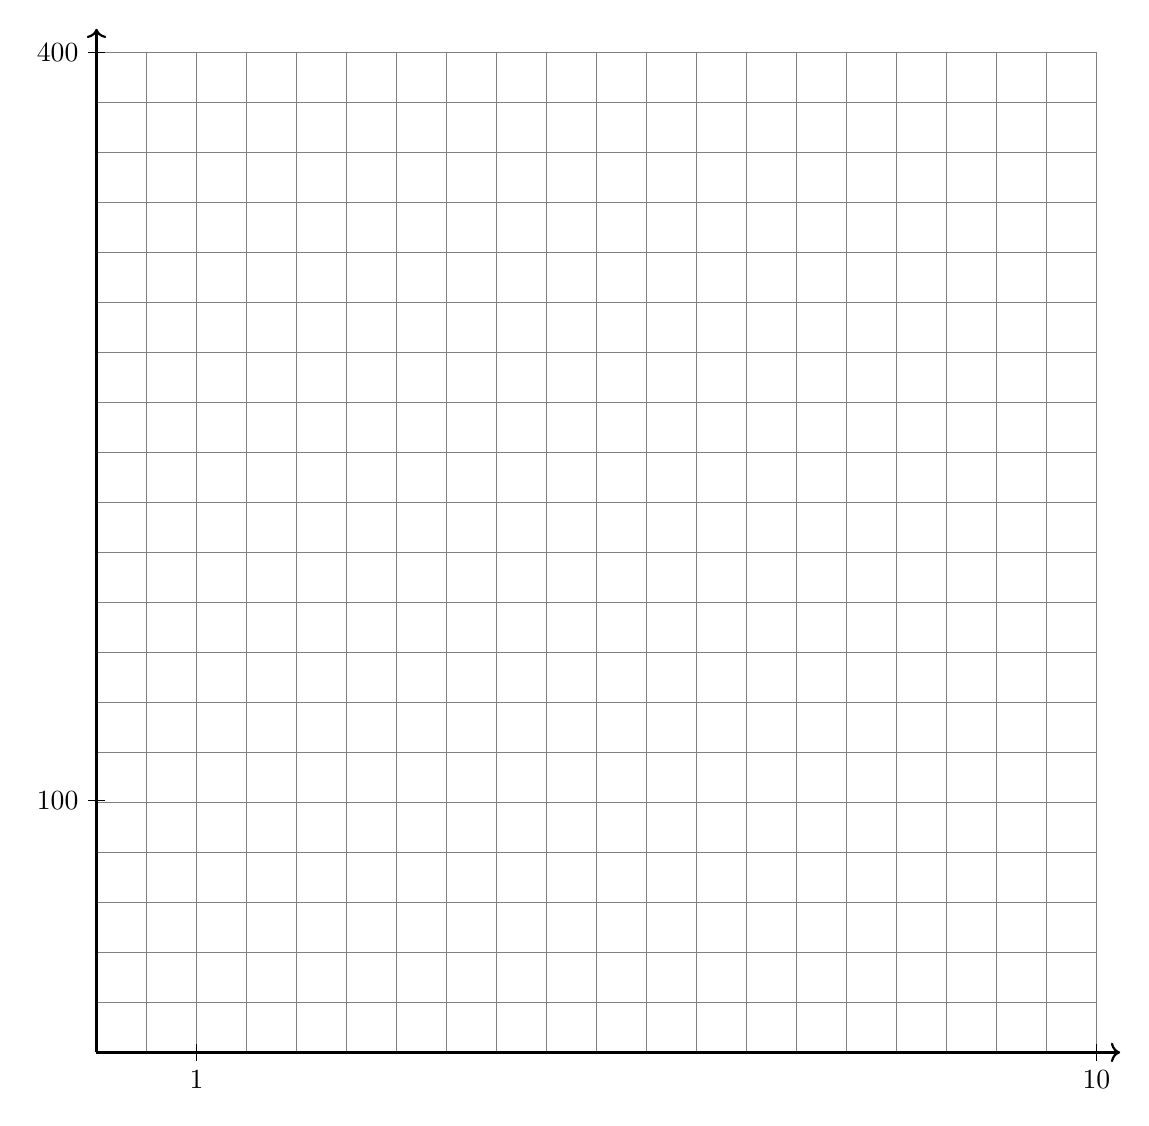
\begin{tikzpicture}
    \draw[step=0.25in,gray,very thin] (0,0) grid (12.7,12.7);
    \draw[thick,->] (0,0) -- (13,0); node[anchor=north west] {x};
    \draw[thick,->] (0,0) -- (0,13); node[anchor=south east] {y};
    \foreach \x in {1.27} \draw (\x cm,3pt) -- (\x cm,-3pt) node[anchor=north] {$1$};
    \foreach \x in {12.7} \draw (\x cm,3pt) -- (\x cm,-3pt) node[anchor=north] {10};
    \foreach \y in {3.2} \draw (3pt,\y cm) -- (-3pt,\y cm) node[anchor=east] {100};
    \foreach \y in {12.7} \draw (3pt,\y cm) -- (-3pt,\y cm) node[anchor=east] {400};
    \end{tikzpicture}
\end{center} %Alg2 Regents Jun2017

\item The value of a certain small passenger car based on its use in years is modeled by $V(t) =28482.698(0.684)^t$, where $V(t)$ is the value in dollars and $t$ is the time in years. Zach had to take out a loan to purchase the small passenger car. The function $Z(t)=22151.327(0.778)^t$, where $Z(t)$ is measured in dollars, and $t$ is the time in years, models the unpaid amount of Zach’s loan over time.\\*[10pt]
Graph $V(t)$ and $Z(t)$ over the interval $0 \leq t \leq 5$, on the set of axes below.
\begin{center}
    
\begin{tikzpicture}
    \draw[step=0.25in,gray,very thin] (0,0) grid (12.7,12.7);
    \draw[thick,->] (0,0) -- (13,0);% node[anchor=north west] {x};
    \draw[thick,->] (0,0) -- (0,13);% node[anchor=south east] {y};
    \end{tikzpicture}
\end{center}
State when $V(t)=Z(t)$, to the \emph{nearest hundredth}, and interpret its meaning in the context of the problem.\\*[10pt]
Zach takes out an insurance policy that requires him to pay a \$3000 deductible in case of a collision. Zach will cancel the collision policy when the value of his car equals his deductible. To the nearest year, how long will it take Zach to cancel this policy? Justify your answer. %Alg2 Regents Aug2017

\newpage
\item Drugs break down in the human body at different rates and therefore must be prescribed by doctors carefully to prevent complications, such as overdosing. The breakdown of a drug is represented by the function $N(t)=N_0(e)^{-rt}$, where $N(t)$ is the amount left in the body, $N_0$ is the initial dosage, $r$ is the decay rate, and $t$ is time in hours. Patient $A, A(t)$, is given 800 milligrams of a drug with a decay rate of 0.347. Patient $B, B(t)$, is given 400 milligrams of another drug with a decay rate of 0.231.\\*[10pt]
Write two functions, $A(t)$ and $B(t)$, to represent the breakdown of the respective drug given to each patient.\\[1in]
Graph each function on the set of axes below.
\begin{center}
    
\begin{tikzpicture}
    \draw[step=0.25in,gray,very thin] (0,0) grid (12.7,12.7);
    \draw[thick,->] (0,0) -- (13,0) node[anchor=north west] {t};
    \draw[thick,->] (0,0) -- (0,13) node[anchor=south east] {y};
    \end{tikzpicture}
\end{center}
%\newpage
To the \emph{nearest hour}, $t$, when does the amount of the given drug remaining in patient $B$ begin to exceed the amount of the given drug remaining in patient $A$?\\*%[3in]
The doctor will allow patient $A$ to take another 800 milligram dose of the drug once only 15\% of the original dose is left in the body. Determine, to the \emph{nearest tenth of an hour}, how long patient $A$ will have to wait to take another 800 milligram dose of the drug. %Alg2 Regents Jun2016
\newpage

\subsubsection*{Topic="Sequences"\\
Source="Regents" 
Difficulty=4}

\item At her job, Pat earns \$25,000 the first year and receives a raise of \$1000 each year. The explicit formula for the $n$th term of this sequence is $a_n = 25,000 + (n - 1)1000$. What rule best represents the equivalent recursive formula?
%Alg2 Regents Jan2018 multiple choice

\item Given $f(9)=2$, which function can be used to generate the sequence  $-8, -7.25, -6.5, -5.75,...$?
\begin{enumerate}
    \item $f(n)=-8+0.75n$
    \item $f(n)=-8-0.75(n-1)$
    \item $f(n)=-8.75+0.75n$
    \item $f(n)=-0.75+8(n-1)$
\end{enumerate} %Alg2 Regents Jun2017 multiple choice

\item The eighth and tenth terms of a sequence are 64 and 100. If the sequence is either arithmetic or geometric, the ninth term can not be
\begin{enumerate}
    \item $-82$
    \item $-80$
    \item 80
    \item 82
\end{enumerate} %Alg2 Regents Jan2017 multiple choice


\subsubsection*{Topic="Series"\\
Source="Regents" 
Difficulty=5}

\item A ball is dropped from a height of 32 feet. It bounces and rebounds 80\% of the height from which it was falling. What is the total downward distance, in feet, the ball traveled up to the 12th bounce? %Alg2 Regents Aug2017 multiple choice

\item Brian deposited 1 cent into an empty non-interest bearing bank account on the first day of the month. He then additionally deposited 3 cents on the second day, 9 cents on the third day, and 27 cents on the fourth day. What would be the total amount of money in the account at the end of the 20th day if the pattern continued? %Alg2 Regents Jan2018 multiple choice


\subsubsection*{Topic="Modeling Trigonometric Functions"\\
Source="Regents" 
Difficulty=3}

\item The volume of air in a person’s lungs, as the person breathes in and out, can be modeled by a sine graph. A scientist is studying the differences in this volume for people at rest compared to people told to take a deep breath. When examining the graphs, should the scientist focus on the amplitude, period, or midline? Explain your choice. %Alg2 Regent Aug2016

\item Relative to the graph of $y=3\sin x$, what is the shift of the graph of $\displaystyle y=3\sin {(x+ \frac{\pi}{3})}$?
\begin{enumerate}
    \item $\frac{\pi}{3}$ right
    \item $\frac{\pi}{3}$ left
    \item $\frac{\pi}{3}$ up
    \item $\frac{\pi}{3}$ down
\end{enumerate} %Alg2 Regent Jan2017


\item As $x$ increases from 0 to $\frac{\pi}{2}$, the graph of the equation $y=2 \tan x$ will
\begin{enumerate}
    \item increase from 0 to 2
    \item decrease from 0 to 2
    \item increase without limit
    \item decrease without limit
\end{enumerate} %Alg2 Regent Aug2017

\item Given the parent function $p(x)=\cos x$, which phrase best describes the transformation used to obtain the graph of $g(x)=  \cos (x+a) - b$, if $a$ and $b$ are positive constants?
\begin{enumerate}
    \item right $a$ units, up $b$ units
    \item right $a$ units, down $b$ units
    \item left $a$ units, up $b$ units
    \item left $a$ units, down $b$ units
\end{enumerate}%Alg2 Regents Jun2017 multiple choice

\item Which equation is represented by the graph shown below?
\begin{center}
    \begin{tikzpicture}[scale=2]
    \draw[thick,<->] (-0.5,0) -- (3.5,0) node[anchor=north west] {\textbf{x}};
    \draw[thick,<->] (0,-1) -- (0,1) node[anchor=south east] {\textbf{y}};
    \foreach \x in {1.57} \draw (\x cm,3pt) -- (\x cm,-3pt) node[anchor=north] {$\frac{\pi}{2}$};
    \foreach \x in {3.14} \draw (\x cm,3pt) -- (\x cm,-3pt) node[anchor=north] {$\pi$};
    \foreach \y in {-0.5, 0.5} \draw (3pt,\y cm) -- (-3pt,\y cm) node[anchor=east] {\y}; %{$\y$};
    \tkzInit[xmin=-.5,xmax=4,ymin=-1,ymax=1,ystep=1]   
    \tkzFct[color=black,very thick,domain = -0.4:3.5] {0.5*cos(2*x)};
    \end{tikzpicture}
\end{center}
\begin{enumerate}
    \item $y=\frac{1}{2} \cos 2x$
    \item $y=\frac{1}{2} \cos x$
    \item $y= \cos x$
    \item $y=2 \cos \frac{1}{2}x$
\end{enumerate} %Alg2 Regents Jun2017 multiple choice

\item The Ferris wheel at the landmark Navy Pier in Chicago takes 7 minutes to make one full rotation. The height, $H$, in feet, above the ground of one of the six-person cars can be modeled by $\displaystyle H(t)=70 \sin{\left( \frac{2 \pi}{7}(t-1.75) \right) +80}$, where $t$ is time, in minutes. Using $H(t)$ for one full rotation, what is this car’s minimum height, in feet? %Alg2 Regents Jun2016

\item The voltage used by most households can be modeled by a sine function. The maximum voltage is 120 volts, and there are 60 cycles \emph{every second}. Which equation best represents the value of the voltage as it flows through the electric wires, where $t$ is time in seconds?
\begin{enumerate}
    \item $V=120 \sin{(t)}$
    \item $V=120 \sin{(60t)}$
    \item $V=120 \sin{(60 \pi t)}$
    \item $V=120 \sin{(120 \pi t)}$
\end{enumerate} %Jun2016 Regents MC

\item The hours of daylight, $y$, in Utica in days, $x$, from January 1, 2013 can be modeled by the equation $y = 3.06 \sin(0.017x-1.40) +12.23$. How many hours of daylight, to the \emph{nearest tenth}, does this model predict for February 14, 2013?

\item On the axes below, graph one cycle of a cosine function with amplitude 3, period $\displaystyle \frac{\pi}{2}$, midline $y=-1$, and passing through the point $(0,2)$.
\begin{center}
    
\begin{tikzpicture}[scale=2.54/4]
    \draw[step=1cm,gray,very thin] (-10,-10) grid (10,10);
    \draw[thick,<->] (-10.5,0) -- (10.5,0) node[anchor=north west] {\textbf{x}};
    \draw[thick,<->] (0,-10.5) -- (0,10.5) node[anchor=south east] {\textbf{y}};
    %\foreach \x in {-6, -4, -2, 2, 4, 6} \draw (\x cm,1pt) -- (\x cm,-1pt) node[anchor=north] {$\x$};
    %\foreach \y in {5} \draw (1pt,\y cm) -- (-1pt,\y cm) node[anchor=east] {50};
    %\foreach \y in {-5} \draw (1pt,\y cm) -- (-1pt,\y cm) node[anchor=east] {-50};    \tkzInit[xmin=-5,xmax=5,ymin=-7,ymax=7,ystep=1]
%    \tkzFct[color=black,thick,<->,domain = -3.4:7] {0.1*(x*x-4)*(x-5)};
    \end{tikzpicture} 
\end{center} %Jun2016 Regents FR

\item Based on climate data that have been collected in Bar Harbor, Maine, the average monthly temperature, in degrees F, can be modeled by the equation $B(x)=23.914 \sin(0.508x-2.116)+55.300$. The same governmental agency collected average monthly temperature data for Phoenix, Arizona, and found the temperatures could be modeled by the equation $P(x)=20.238 \sin(0.525x-2.148)+86.729$.\\*
Which statement can not be concluded based on the average monthly temperature models $x$ months after starting data collection?
\begin{enumerate}
    \item The average monthly temperature variation is more in Bar Harbor than in Phoenix.
    \item The midline average monthly temperature for Bar Harbor is lower than the midline temperature for Phoenix.
    \item The maximum average monthly temperature for Bar Harbor is $79^{\circ}$ F, to the nearest degree.
    \item The minimum average monthly temperature for Phoenix is $20^{\circ}$ F, to the nearest degree.
\end{enumerate} %Alg2 Regents Jun2017 multiple choice

\item The resting blood pressure of an adult patient can be modeled by the function $P$ below, where $P(t)$ is the pressure in millimeters of mercury after time $t$ in seconds.
\[P(t) = 24\cos (3 \pi t) + 120\]
On the set of axes below, graph $y = P(t)$ over the domain $0 \leq t \leq 2$.
\begin{center}
    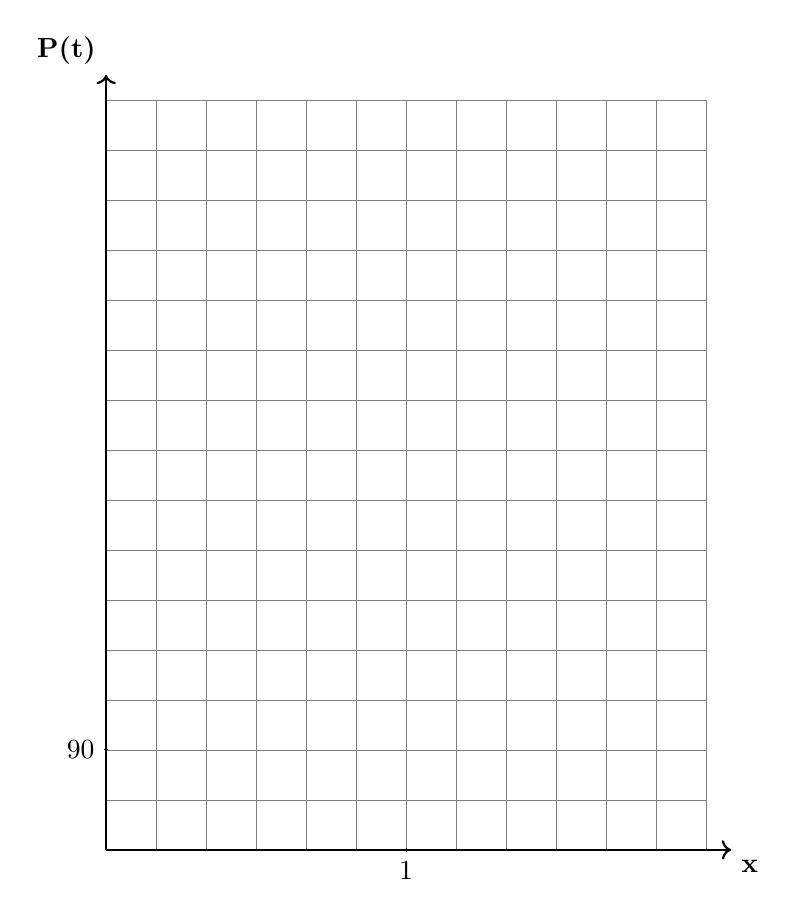
\begin{tikzpicture}[scale=2.54/4]
    \draw[step=1cm,gray,very thin] (0,0) grid (12,15);
    \draw[thick,->] (0,0) -- (12.5,0) node[anchor=north west] {\textbf{x}};
    \draw[thick,->] (0,0) -- (0,15.5) node[anchor=south east] {\textbf{P(t)}};
    \foreach \x in {6} \draw (\x cm,1pt) -- (\x cm,-1pt) node[anchor=north] {1};
    \foreach \y in {2} \draw (1pt,\y cm) -- (-1pt,\y cm) node[anchor=east] {90}; %{$\y$};
    \end{tikzpicture}
\end{center}
Determine the period of $P$. Explain what this value represents in the given context.\\*[10pt]
Normal resting blood pressure for an adult is 120 over 80. This means that the blood pressure oscillates between a maximum of 120 and a minimum of 80. Adults with high blood pressure (above 140 over 90) and adults with low blood pressure (below 90 over 60) may be at risk for health disorders. Classify the given patient’s blood pressure as low, normal, or high and explain your reasoning.



\item Consider the function $h(x) = 2\sin(3x) + 1$ and the function $q$ represented in the table below.\\*
\begin{center}
\begin{tabular}{|c|c|}
    \hline 
    $\boldsymbol{x}$ & $\boldsymbol{q(x)}$\\ 
    \hline 
    -2 & -8 \\ 
    \hline 
    -1 & 0 \\ 
    \hline 
    0 & 0 \\ 
    \hline 
    1 & -2 \\ 
    \hline 
    2 & 0 \\ 
    \hline 
\end{tabular}\\*[5pt]
\end{center}
Determine which function has the \emph{smaller} minimum value for the domain $[-2,2]$. Justify your answer. %Alg2 Regents Jan2018

\item a) On the axes below, sketch at least one cycle of a sine curve with an amplitude of 2, a midline at $\displaystyle y = -\frac{3}{2}$, and a period of $2\pi$. 
\begin{center}
    \begin{tikzpicture}[scale=0.8]
    \draw[thick,<->] (-7.5,0) -- (7.5,0) node[anchor=north west] {\textbf{x}};
    \draw[thick,<->] (0,-7.5) -- (0,7.5) node[anchor=south east] {\textbf{y}};
    \end{tikzpicture}
\end{center}
b) Explain any differences between a sketch of $\displaystyle y = 2 \sin \left( x- \frac{\pi}{3} \right) -\frac{3}{2}$ and the sketch from part $a$. %Alg2 Regents Aug2017

\subsubsection*{Topic="Evaluating Radical Expressions"\\ %may not be a category
Source="Regents"\\
Difficulty=6}

\item Solve the equation $\sqrt{2x-7}+x=5$ algebraically, and justify the solution set.
 %Alg2 Regents Aug2016

\item The speed of a tidal wave, $s$, in hundreds of miles per hour, can be modeled by the equation $s= \sqrt{t} - 2t+6$, where $t$ represents the time from its origin in hours. Algebraically determine the time when $s=0$.\\[10pt]
How much faster was the tidal wave traveling after 1 hour than 3 hours, to the \emph{nearest mile per hour}? Justify your answer. %Alg2 Regents Jan2017

\subsubsection*{Topic="Evaluating Logarithmic Expressions"\\
Source="IB"\\
Difficulty=4}


\item Let $\log_3 p = 6$ and $\log_3 q = 7$.
\begin{enumerate}
    \item Find $\log_3 {p^2}$
    \item Find $\displaystyle \log_3 {\left( \frac{p}{q} \right) }$
    \item Find $\log_3 {(9p)}$
\end{enumerate}

Difficulty=5
\item If $ae^{bt}=c$, where $a$, $b$, and $c$ are positive, then $t$ equals what? %Alg2 Regents Jan2018 multiple choice

\item What is the solution to $8(2^{x+3})=48$? %Alg2 Regents Jun2017 multiple choice

\item To the \emph{nearest tenth}, what is the value of $x$ that satisfies $2^x=-2x+11$? %Alg2 Regents Aug2016 MC

Calc=2
\item For which values of $x$, rounded to the \emph{nearest hundredth}, will $|x^2-9|-3= \log_3 x$?  %Alg2 Regents Jan2018 multiple choice

\item When $\displaystyle g(x)= \frac{2}{x+2}$ and $h(x)=\log (x+1) +3$ are graphed on the same set of axes, what coordinate pair represents their point of intersection? %Alg2 Regents Jan2017 multiple choice

\item If $f(x)=3|x| -1$ and $g(x)= 0.03x^3 -x +1$, an approximate solution for the equation $f(x)= g(x)$ is
\begin{enumerate}
    \item $1.96$
    \item $11.29$
    \item $(-0.99, 1.96)$
    \item $(11.29, 32.87)$
\end{enumerate}

\item The $x$-value of which function's $x$-intercept is larger, $f$ or $h$? Justify your answer. \[f(x)=\log (x-4) \]
\begin{tabular}{|c|c|}
\hline 
x & h(x)\\ 
\hline 
$-1$ & 6 \\ 
\hline 
0 & 4 \\ 
\hline 
1 & 2 \\ 
\hline 
2 & 0 \\ 
\hline 
3 & $-2$ \\ 
\hline 
\end{tabular} %Alg2 Regents Aug2016

\subsubsection*{Topic="Graphing Logarithmic Functions"\\
Source="IB" 
Difficulty=5 
Calc=2}

\item Which statement about the graph of $c(x)= \log_6{x}$ is false?
\begin{enumerate}
    \item The asymptote has equation $y=0$.
    \item The graph has no $y$-intercept.
    \item The domain is the set of positive reals.
    \item The range is the set of all real numbers.
\end{enumerate}

\item Graph $y= \log_2(x+3)-5$ on the set of axes below. Use an appropriate scale to include both intercepts.
\begin{center}
    
\begin{tikzpicture}[scale=2.54/4]
    \draw[step=1cm,gray,very thin] (-10,-10) grid (10,10);
    \draw[thick,<->] (-10.5,0) -- (10.5,0) node[anchor=north west] {\textbf{x}};
    \draw[thick,<->] (0,-10.5) -- (0,10.5) node[anchor=south east] {\textbf{y}};
%    \foreach \x in {-2, 2} \draw (\x cm,1pt) -- (\x cm,-1pt) node[anchor=north] {$\x$};
%    \foreach \y in {5} \draw (1pt,\y cm) -- (-1pt,\y cm) node[anchor=east] {50}; %{$\y$};
%    \tkzInit[xmin=-5,xmax=5,ymin=-7,ymax=7,ystep=1]   
%    \tkzFct[color=black,thick,<->,domain = -4.4:3.6] {0.1*(x+4)*x*x*(x-3)};
    \end{tikzpicture}
\end{center}

Describe the behavior of the given function as $x$ approaches $-3$ and as $x$ approaches positive infinity. %Alg2 Regents Jun2017 

\subsubsection*{Topic="Experimental design - not actual category"\\
Source="Regents" 
Difficulty=4 
Calc=1}

\item Which statement about statistical analysis is \emph{false}?
\begin{enumerate}
    \item Experiments can suggest patterns and relationships in data.
    \item Experiments can determine cause and effect relationships.
    \item Observational studies can determine cause and effect relationships.
    \item Observational studies can suggest patterns and relationships in data.
\end{enumerate} %Alg2 Regents Jan2017 MC

\item Describe how a controlled experiment can be created to examine the effect of ingredient $X$ in a toothpaste. %Regents Jun2016
%A correct description of a controlled experiment is written, such as indicating two randomly assigned groups, one with ingredient X and one without ingredient X. ("control group, randomly assigned, with/without")

\item An orange-juice processing plant receives a truckload of oranges. The quality control team randomly chooses three pails of oranges, each containing 50 oranges, from the truckload. Identify the sample and the population in the given scenario.\\[1.5in]
State \emph{one} conclusion that the quality control team could make about the population if 5\% of the sample was found to be unsatisfactory. %Alg2 Regents Jan2017

\subsubsection*{Topic="Probability of Compound Events"\\
Source="IB" 
Difficulty=4 
Calc=1}

\item Two events $A$ and $B$ are such that $P(A)=0.2$ and $P(A \cup B) =0.5$. 
\begin{enumerate}
    \item Given that $A$ and $B$ are mutually exclusive, find $P(B)$.
    \item Given that $A$ and $B$ are independent, find $P(B)$.
\end{enumerate}

\item Given events $A$ and $B$, such that $P(A)= 0.6$, $P(B) = 0.5$, and $P(A \cup B)=0.8$, determine whether $A$ and $B$ are independent or dependent. %Regents Alg2 Aug2016

\item Sean’s team has a baseball game tomorrow. He pitches 50\% of the games. There is a 40\% chance of rain during the game tomorrow. If the probability that it rains given that Sean pitches is 40\%, it can be concluded that these two events are
\begin{enumerate}
    \item independent
    \item dependent
    \item mutually exclusive
    \item complements
\end{enumerate} %Regents Alg2 Jun2016 MC

\item The probability that Gary and Jane have a child with blue eyes is 0.25, and the probability that they have a child with blond hair is 0.5. The probability that they have a child with both blue eyes and blond hair is 0.125. Given this information, the events blue eyes and blond hair are\\*
.\qquad I: dependent\\*
.\qquad II: independent\\*
.\qquad III: mutually exclusive\\* %Alg2 Regents Jun2017 multiple choice

\item Data collected about jogging from students with two older siblings are shown in the table below.\\*[5pt]
\begin{tabular}{|c|c|c|c|}
\hline 
& Neither Sibling & One Sibling & Both Siblings\\ 
& Jogs & Jogs & Jogs\\\hline 
Student Does Not Jog & 1168 & 1823 & 1380 \\ 
\hline 
Student Jogs & 188 & 416 & 400 \\ 
\hline 
\end{tabular}\\*[5pt]
Using these data, determine whether a student with two older siblings is more likely to jog if one sibling jogs or if both siblings jog. Justify your answer. %Alg2 Regents Jun2017

\item A student is chosen at random from the student body at a given high school. The probability that the student selects Math as the favorite subject is $\frac{1}{4}$. The probability that the student chosen is a junior is $\frac{116}{459}$. If the probability that the student selected is a junior or that the student chooses Math as the favorite subject is $\frac{47}{108}$, what is the exact probability that the student selected is a junior whose favorite subject is Math?\\*[15pt]

Are the events ``the student is a junior” and ``the student’s favorite subject is Math” independent of each other? Explain your answer. %Alg2 Regents Jan2018

\subsubsection*{Topic="Conditional Probability"\\
Source="IB" 
Difficulty=5 
Calc=1}

\item Given events $A$ and $B$, such that $\mathrm \mathrm P(A)=0.6, \mathrm P(B)=0.5$, and $\mathrm P(A \cup B) =0.8$, determine whether $A$ and $B$ are dependent or independent. Justify your answer.

Difficulty=6 
\item A study was designed to test the effectiveness of a new drug. Half of the volunteers received the drug. The other half received a sugar pill. The probability of a volunteer receiving the drug and getting well was 40\%. What is the probability of a volunteer getting well, given that the volunteer received the drug? %Alg2 Regents Aug2017

\subsubsection*{Topic="Normal Distributions"\\
Source="IB" 
Difficulty=4 
Calc=2}

\item The random variable $X$ is normally distributed with mean 20 and standard deviation 5. 
\begin{enumerate}
    \item Find $P(X \leq 22.9)$.
    \item Given that $P(X < k) = 0.55$, find the value of $k$.
\end{enumerate}

Source="Regents" 
Difficulty=4 
Calc=2

\item There are 440 students at Thomas Paine High School enrolled in U.S. History. On the April report card, the students’ grades are approximately normally distributed with a mean of 79 and a standard deviation of 7. Students who earn a grade less than or equal to 64.9 must attend summer school. Approximately how many students must attend summer school for U.S. History?

\item A suburban high school has a population of 1376 students. The number of students who participate in sports is 649. The number of students who participate in music is 433. If
the probability that a student participates in either sports or music is $\displaystyle \frac{974}{1376}$, what is the probability that a student participates in both sports and music? %Alg2 Regents Jun2016

\subsubsection*{Topic="Using Trigonometry to Find Area"\\
Source="IB" 
Difficulty=4 
Calc=2}

\item The area of triangle ABC is 80 sq. cm, AB = 18 cm, AC = $x$ cm and B\^AC = $50^\circ$. Find $x$.


\subsubsection*{Differentiate each function.}

\item $f(x)=2x^3-x^2+6$
\item $g(x) = \frac{1}{x^4}$
\item $h(x)= 3\sqrt{x}$
\item $f(x)=(x-2)(x+2)$
\item $g(x)=\frac{2}{(3x)^2}$
\item $h(x)=6e^x+\sqrt{x^3}$
\item $f(x)=6\ln{x}$
\item $g(x) = \displaystyle \frac{\sin x}{\pi}$
\item $h(x)= \log_3{x}$

\subsubsection*{Find the equation of the tangent or normal line to the function at the given point.}

\item The tangent to $y=4x^2$ at $x=1$
\item The tangent to $y=3x^2-e^x$ at $x=2$
\item The normal line to $\displaystyle y=\ln(e^{x^2})$

\subsubsection*{Use the product, quotient, or chain rule to differentiate each function.}

\item $y=2xe^x$
\item $y= x^2\cos{x}$
\item $f(x)= \displaystyle \frac{x^2-8}{x+1}$
\item $g(x) =\displaystyle \frac{x}{x^2-x+6}$
\item $y = (3x^3-x^2+4)^4$
\item $y= \ln{2x^2-3x}$
\item $y= \displaystyle \cos{\frac{x^3}{\pi}}$
\item $y = \sqrt{\cos{3x}}$

\subsubsection*{Local extrema: find the value(s) of $x$ for which the function has a local minimum or maximum.}

\item $f(x) = 8x^2-24x+7$.
\item $g(x) = x^3-4x^2-6x+5$
\item $h(x) = 2\ln x - x+4$


\subsubsection*{Rates of change and motion equations}

\item The path of a diver is modeled by the function $s(t)=-4.9t^2+4.9t+10$ where $s$ is the diver's height above the water in meters. 
\begin{enumerate}
    \item What is the initial height from which the diver begins her dive?
    \item What is the initial velocity of the diver?
    \item What is the maximum height above the water and at what point in time is that height reached?
    \item When does the diver enter the water? 
    \item At what velocity does she enter the water?
\end{enumerate}

\item The position of an object is given by the function $s(x) = 5\sin x +x$ over the interval $\{0\leq x  \leq 2\pi \}$
\begin{enumerate}
    \item What is the object's initial velocity?
    \item At what value of $x$ is the object at its maximum distance from its starting point? 
    \item What is its average velocity over the period from $x=0$ to when it achieves its maximum distance? 
    \item Over what interval is the object moving in the negative direction?
\end{enumerate}


\item A particle moves along a horizontal line with its displacement given by the function $s(t) = 20t - 100 \ln{t}$, for $t>1$.
\begin{enumerate}
    \item Find the velocity of the particle.
    \item Over what period is the particle moving to the left?
    \item Show that the velocity of the particle is always increasing.
\end{enumerate}

\subsubsection*{Unit conversions}

\item The two common systems of temperature measurement, Fahrenheit and Celsius, are based on the freezing and boiling points of water. In the Fahrenheit system, water freezes at $32 \ ^\circ\text{F}$ and boils at $212 \ ^\circ\text{F}$. In the Celsius (or centigrade) system, the freezing and boiling points of water are $0 \ ^\circ \text{C}$ and $100 \ ^\circ \text{C}$, respectively.
\begin{enumerate}
    \item Show that $\displaystyle 1 \ ^\circ \text{C} = \frac{9}{5} \ ^\circ \text{F}$.
    \item On the graph below, plot and label the freezing and boiling points of water, and draw a straight line representing the mapping $^\circ \text{F}\to \ ^\circ \text{C}$.
    \item What is the Fahrenheit equivalent of $20 \ ^\circ \text{C}$? Label it on the graph as ``room temperature."
    \item Determine an algebraic expression for a temperature in Celsius, $C(x)$, as a function of the temperature in Fahrenheit, $x$.
    \item Solve for the temperature for which the Fahrenheit and Celsius measures are the same, that is, $C(x)=x$.
\end{enumerate}

\end{enumerate}
\end{document}